\documentclass{article}
\usepackage{amsmath}
\usepackage{amssymb}
\usepackage{array}
\usepackage{booktabs}
\usepackage{textcomp}
\usepackage{graphicx}
\usepackage{tikz}
\usepackage{graphics}
\usepackage{pdfpages}

\usepackage{amsthm}
\newtheorem{theorem}{Theorem}[section]

\newtheorem{lemma}[theorem]{Lemma}



\newcommand{\coNP}{\textrm{co-}\mathbb{NP}}

\title{hw2}
\author{Ian Chi}
\date{\today}
\begin{document}
\maketitle
\section{}

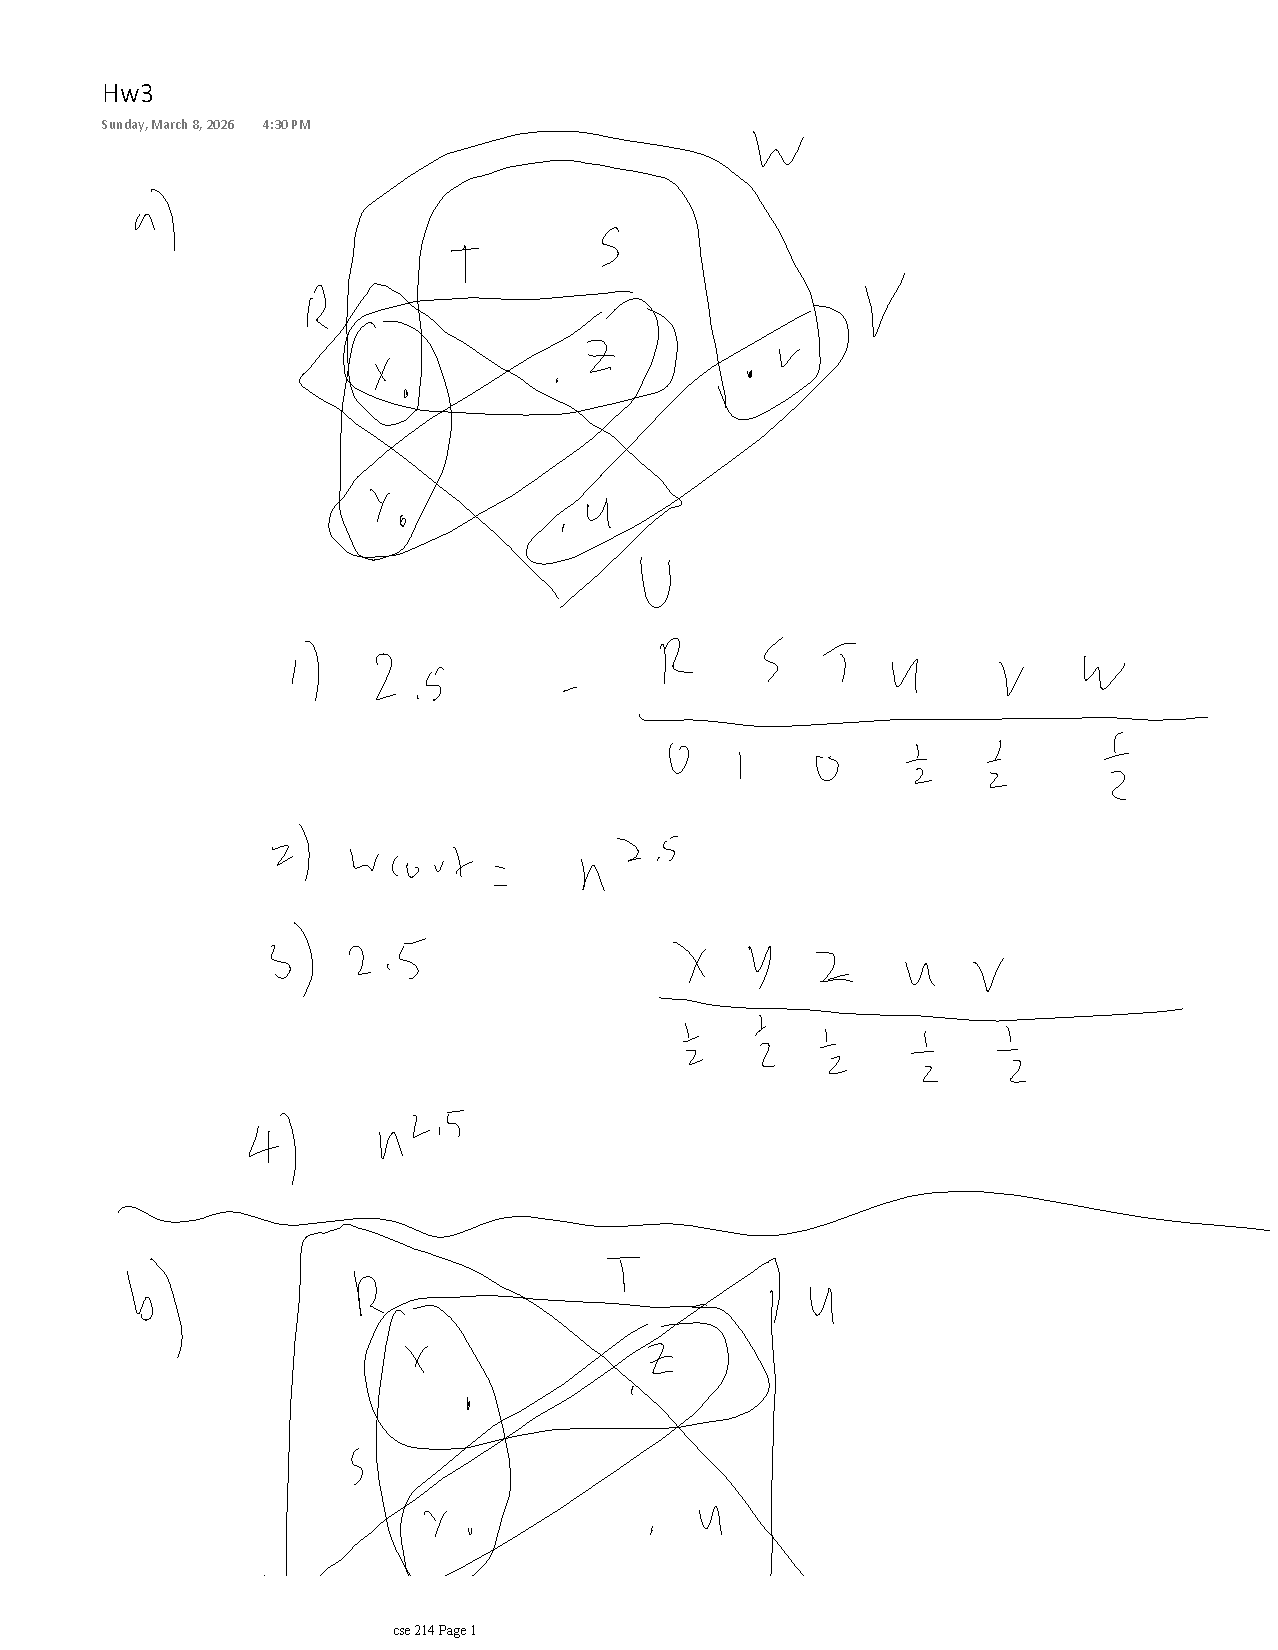
\includepdf[pages=1-2]{Hw3_onenote.pdf}

% \begin{enumerate}
%     % \item 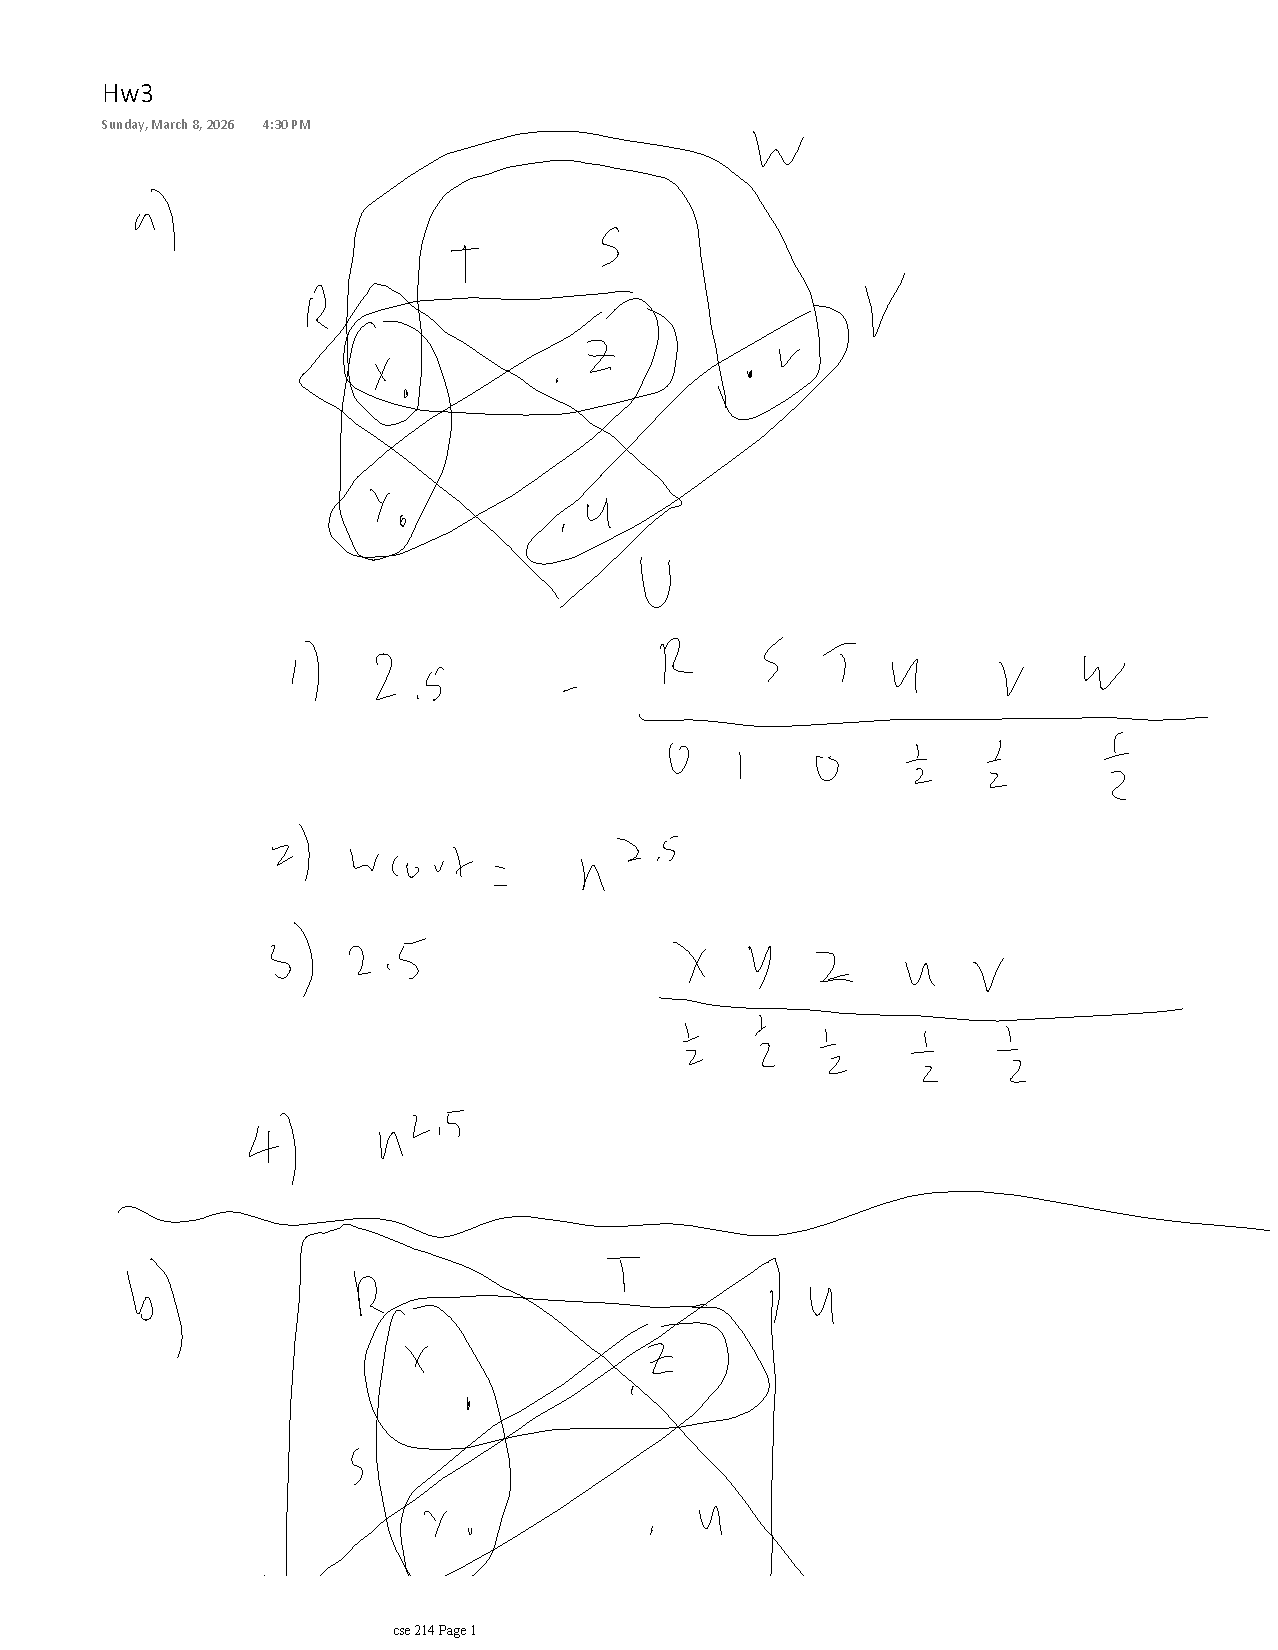
\includegraphics[width=1.0\textwidth]{Hw3.pdf}
% \end{enumerate}

\newpage
\section{}
\begin{enumerate}
    \item the width does not depend on k. the width remains 2 for all \(k\geq 3\)
    \item 
    \begin{verbatim}
SELECT COUNT(*)
FROM edges e1
JOIN edges e2 ON e1.dst = e2.src
JOIN edges e3 ON e2.dst = e3.src
JOIN edges e4 ON e3.dst = e4.src
WHERE e4.dst = e1.src;
    \end{verbatim}
    178704122
    this took 42437.452 ms (00:42.437)
    \item 
    \begin{verbatim}
        WITH
p23 AS (
    SELECT e1.src AS x2, e1.dst AS x3, e2.dst AS x4
    FROM edges e1
    JOIN edges e2 ON e1.dst = e2.src
),

p1234 AS (
    SELECT e.src AS x1, p.x2, p.x3, p.x4
    FROM edges e
    JOIN p23 p ON e.dst = p.x2
),

cycles AS (
    SELECT *
    FROM p1234 p
    JOIN edges e ON p.x4 = e.src AND e.dst = p.x1
)

SELECT COUNT(*) FROM cycles;
    \end{verbatim}
     178704122
    Time: 44329.151 ms (00:44.329)

\end{enumerate}

it took almost the same amount of time, slightly longer. it has some overhead i guess?



\end{document}